\documentclass[border=10pt]{standalone}

\usepackage{tikz}
\usepackage{tikzsymbols}
\usetikzlibrary{calc,patterns,shapes.geometric}

\def\centerarc[#1](#2)(#3:#4:#5){\draw[#1] ($(#2)+({#5*cos(#3)},{#5*sin(#3)})$) arc (#3:#4:#5);}

\begin{document}
	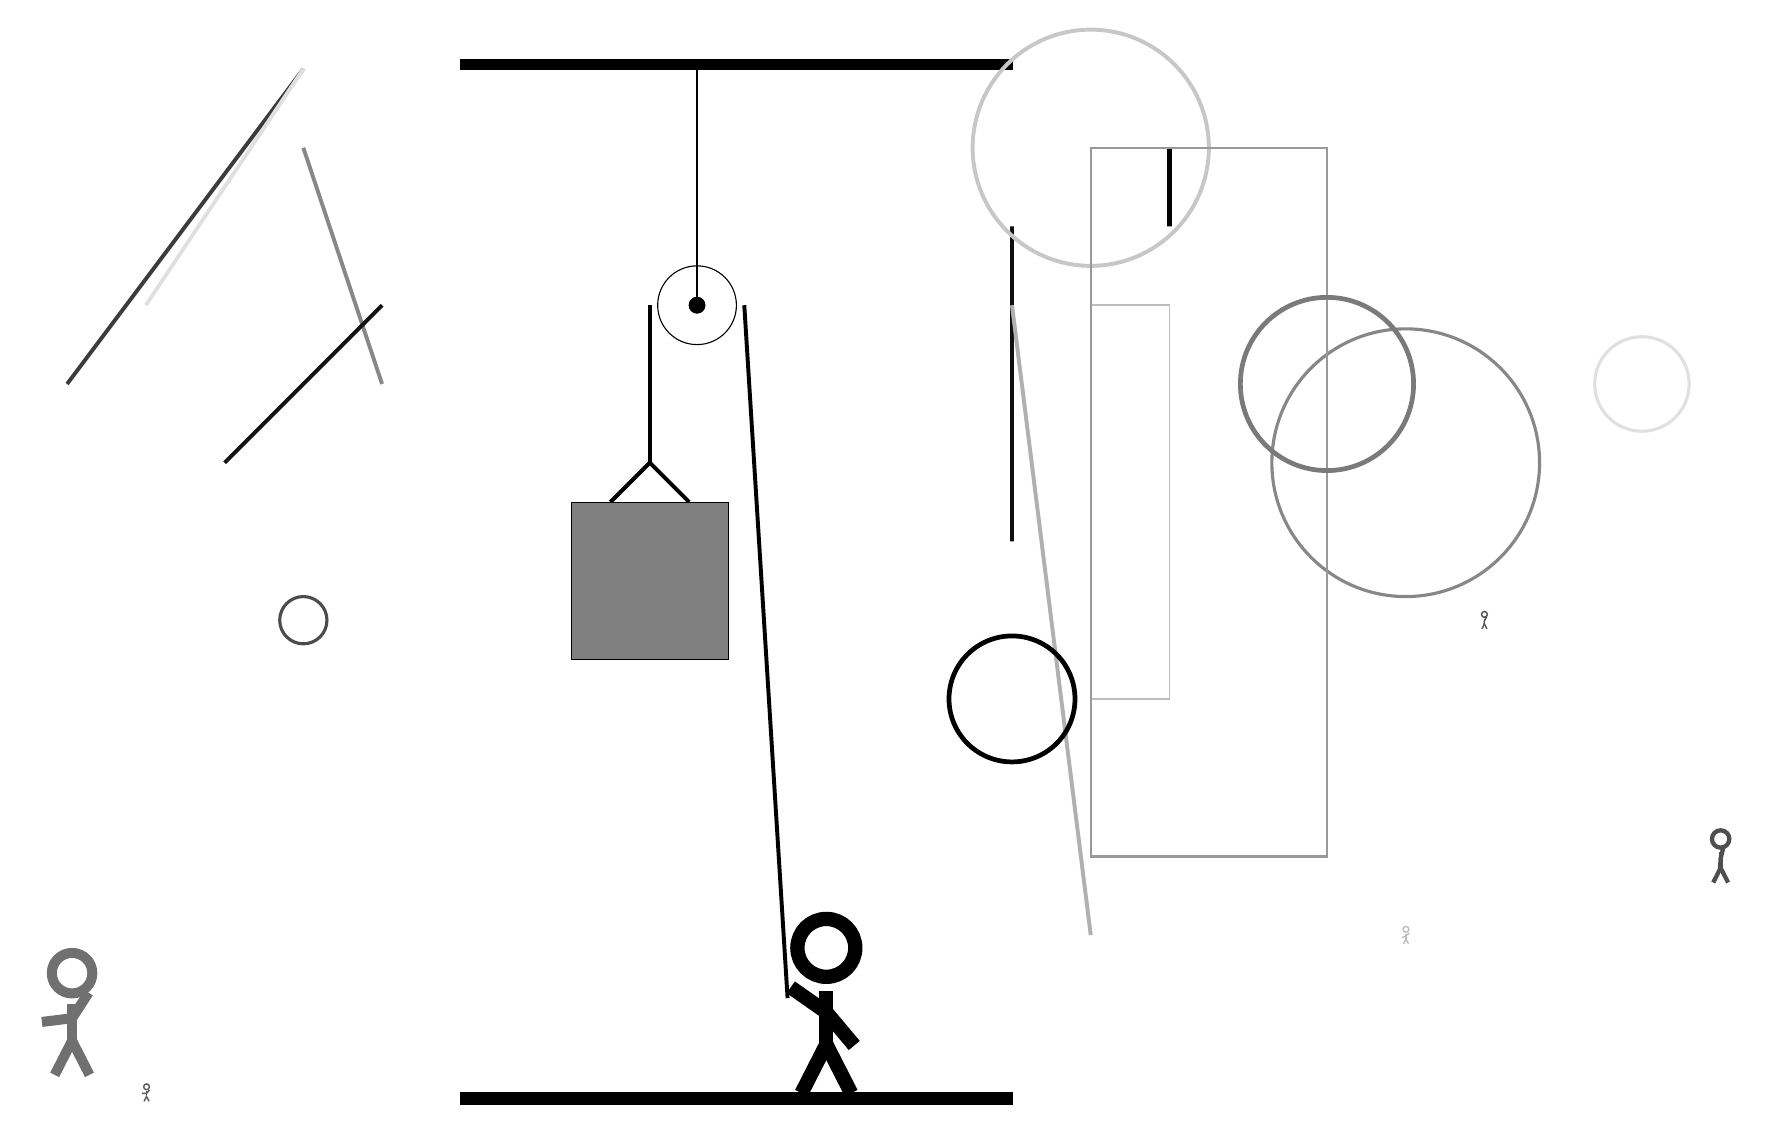
\begin{tikzpicture}
		%%%%% START %%%%%
		
		\draw[fill=black] (-2, 10) rectangle (5, 10.125);
		
		\draw[line width=0.5mm, color=black!47](-4, 9) -- (-3, 6);
		
		\node[line width=0.2mm, color=black!68] at (11, 3) {\Strichmaxerl[1][84][62]};
		\draw[line width=0.5mm, color=black!94] (5, 4) rectangle (5, 8);
		\node[line width=0.7mm, color=black!64] at (-6, -3) {\Strichmaxerl[1][2][47]};
		
		\draw[line width=0.5mm, color=black!31](5, 7) -- (6, -1);
		
		\draw[line width=0.7mm, color=black!99] (7, 9) rectangle (7, 8);
		\draw [line width=0.5mm, color=black!22](6, 9) circle (1.5);
		
		\draw[line width=0.5mm, color=black!92](-3, 7) -- (-5, 5);
		\node[line width=0.4mm, color=black!56] at (-7, -2) {\Strichmaxerl[7][7][57]};
		\node[line width=0.7mm, color=black!69] at (14, 0) {\Strichmaxerl[3][86][76]};
		\draw[line width=0.2mm, color=black!26] (6, 2) rectangle (7, 7);
		\draw [line width=0.4mm, color=black!47](10, 5) circle (1.7);
		\draw [line width=0.4mm, color=black!70](-4, 3) circle (0.3);
		
		\draw[line width=0.5mm, color=black!77](-7, 6) -- (-4, 10);
		\draw [line width=0.6mm, color=black!100](5, 2) circle (0.8);
		\draw [line width=0.4mm, color=black!12](13, 6) circle (0.6);
		
		\draw[line width=0.3mm, color=black!40] (6, 9) rectangle (9, 0);
		\draw[line width=0.5mm, color=black!12](-4, 10) -- (-6, 7);
		\draw [line width=0.6mm, color=black!52](9, 6) circle (1.1);
		
		\node[line width=0.4mm, color=black!26] at (10, -1) {\Strichmaxerl[1][25][40]};
		
		\draw (1, 7) circle (0.5);
		\draw[fill=black] (1, 7) circle (0.1);
		\draw (1, 10) -- (1, 7);
		
		\draw[line width=0.5mm] (-0.1, 4.5) -- (0.4, 5.0) -- (0.9, 4.5);
		\draw[fill=black!50] (-0.6, 4.5) rectangle (1.4, 2.5);
		
		\draw[line width=0.5mm] (0.4, 7) -- (0.4, 5.0);
		\centerarc[line width=0.5mm](1, 7)(0:180:0.6);
		\draw[line width=0.5mm](1.6, 7) -- (2.15, -1.8);
		
		\node at (2.6, -1.9) {\Strichmaxerl[10][-35][-50]};
		
		\draw[fill=black] (-2, -3) rectangle (5, -3.15);
		
		%%%%% END %%%%%
	\end{tikzpicture}
\end{document}